null
\chapter{DESENVOLVIMENTO DO PROJETO}

\bigskip


A metodologia de\ \textit{Extreme Programming}\ (XP) foi escolhida, devido ao fato de estar muito relacionada a
agilidade e flexibilidade, caracter\'isticas essas que\ condiziam com a forma como desej\'avamos trabalhar.

Logo em seguida notamos que, antes de iniciar o desenvolvimento do software, dever\'iamos dividir nossa equipe em tr\^es
frentes de trabalho, para que pud\'essemos desenvolver o projeto com mais agilidade e efici\^encia. Elas se
comunicariam com frequ\^encia e trocariam suas experi\^encias pesquisas e conclus\~oes a cada etapa que fosse superada.
As tr\^es frentes de trabalho que eram divididas em A, B e C tinham as seguintes fun\c{c}\~oes:


\bigskip

\liststyleLFOi
\begin{itemize}
\item {
Frente de trabalho A: Verificar quais\ as exig\^encias da Metodista em rela\c{c}\~ao \`a padroniza\c{c}\~ao ABNT e
planejar como nosso software ira auxiliar o usu\'ario a atender essas exig\^encias.}
\item {
\textrm{Frente de trabalho B: Pesquisar como funciona a metodologia escolhida para desenvolver o software e preparar a
equipe do projeto para aplicar essa metodologia.}}
\item {
\textrm{Frente de trabalho C: Pesquisar e aprender como utilizar as tecnologias que iriam permitir o desenvolvimento do
TCCTeX e como seria feita a intera\c{c}\~ao dessas tecnologias.\ }}
\end{itemize}

\bigskip

Essas tr\^es frentes de trabalho foram, como previsto, naturalmente se complementando e conforme as atividades de uma
frente avan\c{c}avam elas alcan\c{c}avam um n\'ivel o qual dependeriam da intera\c{c}\~ao com outra frente de trabalho
para se desenvolver.\ 

A primeira frente de trabalho que alcan\c{c}ou esse n\'ivel foi a frente de trabalho A que conseguiu captar as
necessidades que o software deveria suprir e planejar como ele iria interagir com o usu\'ario desenvolvendo
prot\'otipos visuais do TCCTeX. A partir dessa conclus\~ao a frente de trabalho A passou a trabalhar em\ conjunto com a
frente C para encontrar as tecnologias e ferramentas que viabilizariam o desenvolvimento do software dentro desses
par\^ametros e discutir poss\'iveis altera\c{c}\~oes dos prot\'otipos em prol de melhorias nas funcionalidades do
TCCTeX.

Em seguida a frente de trabalho B conseguiu estabelecer como iriamos aplicar a metodologia XP em nosso projeto e passou
a toda a equipe do projeto como seriam implantada a metodologia e como ela iria auxiliar no desenvolvimento do
software.\ 


A frente de trabalho C, por\ sua vez conseguiu encontrar diversas tecnologias que poderiam possibilitar no
desenvolvimento do software e passou a testa-las para verificar a efici\^encia de cada uma delas e escolher quais
melhor se adequavam com as necessidades do software. A frente de trabalho C s\'o concluiria esse processo de pesquisa e
escolha durante o desenvolvimento do software, pois seria durante o desenvolvimento do software que essas tecnologias e
a capacidade de intera\c{c}\~ao delas seriam realmente posta a prova.


\bigskip

\section{APLICA\c{C}\~AO DA METODOLOGIA XP}

\bigskip

Com base em nossos estudos sobre Extreme Programming (XP) notamos que essa metodologia requer contato direto e
recorrente do cliente do projeto em desenvolvimento e neste quesito notamos uma diferen\c{c}a entre o nosso projeto e
outros projetos desenvolvidos utilizando XP, pois como alunos da Universidade Metodista de S\~ao Paulo, n\'os podemos
assumir o papel tanto de clientes desse projeto como de desenvolvedores do mesmo.


A partir do momento em que come\c{c}amos a aplicar XP na pr\'atica tivemos que nos conscientizar dos dois pap\'eis que
exercemos e como lidar com essa dualidade sem prejudicar o andamento do projeto nem no produto final.


Para suprir a impossibilidade da equipe de nos reunir e compartilhar um espa\c{c}o de trabalho \'unico, portanto, n\~ao
termos um local f\'isico para colocarmos um quadro de tarefas ou de cart\~oes de hist\'oria, utilizamos a ferramenta de
anota\c{c}\~oes Microsoft Office OneNote combinado com o servi\c{c}o de armazenamento e partilha de arquivos Dropbox.
Essa uni\~ao nos possibilitou a flexibilidade do\ planejamento do projeto tal qual \'e previsto na metodologia XP.\ 

Para iniciar o projeto aplicando XP dever\'iamos assumir o papel de clientes e escrever cart\~oes de\ hist\'oria (User
Stories) contando o que um aluno da UMESP que est\'a desenvolvendo a documenta\c{c}\~ao\ do seu TCC deseja que o
software TCCTeX fa\c{c}a por ele. Para escrever as hist\'orias de usu\'ario t\'inhamos o seguinte modelo:


\bigskip




\begin{figure}[H]
\caption{Modelo de User Stories}
 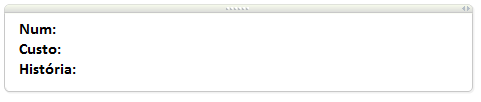
\includegraphics[width=5.01319in,height=1.06528in]{Cap03-img/Cap03-img001.png} 
\fonte{Autoria pr\'opria}} 
\end{figure}





\bigskip

O qual deveria ser usado seguindo a seguinte referencia:

\liststyleLFOii
\begin{itemize}
\item {
\textbf{Num:}\ n\'umero de\ identifica\c{c}\~ao do cart\~ao.}
\item {
\textbf{Custo:\ }estimativa de custo de tempo de 1 \`a 3 semanas que deve ser feita em grupo.}
\item {
\textbf{Hist\'oria:}\ n\'os, no papel de clientes, dever\'iamos escrever hist\'orias de o que gostar\'iamos que o
software fizesse\ evitando termos t\'ecnicos.}
\end{itemize}

\bigskip

Cada uma dessas hist\'orias representa uma parte de software que pode ser entregue a parte.\ Ap\'os escrever as
hist\'orias n\'os em grupo, assumindo o papel de desenvolvedores dever\'iamos fazer uma Reuni\~ao de Planejamento de
Releases (entregas, libera\c{c}\~oes do software) onde estim\'avamos o tempo que levar\'iamos para transformar cada uma
dessas hist\'orias em c\'odigo e em seguida escolh\'iamos quais hist\'orias desenvolver\'iamos primeiro.

Estas hist\'orias eram organizadas, j\'a na ordem de desenvolvimento em um documento do One Note chamado Plano de
Libera\c{c}\~ao que continha tamb\'em os Testes Funcionais que eram desenvolvidos durante as\ Reuni\~oes de
Planejamento de Itera\c{c}\~oes.

Os\ Testes Funcionais representam o resultado esperado do sistema. Cada hist\'oria possui um ou mais Testes Funcionais
que eram\ ser aplicados para verificar se essa hist\'oria foi completamente implementada. Cada um dos Testes Funcionais
possu\'ia uma caixa de sele\c{c}\~ao que tinham a seguinte fun\c{c}\~ao:


\bigskip



\begin{figure}[H]
\caption{Caixa de Sele\c{c}\~ao dos Testes Funcionais}
 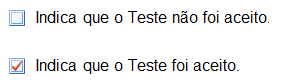
\includegraphics[width=2.97431in,height=0.87014in]{Cap03-img/Cap03-img002.png} 
\fonte{Autoria pr\'opria}} 
\end{figure}

\bigskip


Fizemos Testes Funcionais simples e de f\'acil verifica\c{c}\~ao visual.

Decidimos que far\'iamos itera\c{c}\~oes de uma semana com Reuni\~oes de Planejamento de Itera\c{c}\~ao no inicio de
cada semana. As reuni\~oes tinham como objetivo dividir hist\'orias em tarefas, decidir quais tarefas seriam
desenvolvidas durante a semana e escrever\ Testes Funcionais. Faz\'iamos tamb\'em reuni\~oes ao final de cada semana
que eram utilizadas para verificar os resultados da semana e propor poss\'iveis novas tarefas a partir das
experi\^encias da semana que se passou.

As tarefas que s\~ao planejadas s\~ao escritas seguindo o seguinte modelo:

\bigskip


\begin{figure}[H]
\caption{Modelo de Cart\~ao de Tarefa}
 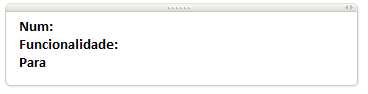
\includegraphics[width=3.83125in,height=0.97431in]{Cap03-img/Cap03-img003.png} 
\fonte{Autoria pr\'opria}} 
\end{figure}

\bigskip

O qual deveria ser usado seguindo a seguinte referencia:

\liststyleLFOii
\begin{itemize}
\item {
\textbf{Num:}\ neste campo ser\'a colocado um numero ser\'a utilizado para\ fazer a referencia entre o cart\~ao de
hist\'oria de usu\'ario e cada tarefa.}
\item {
\textbf{Funcionalidade:}\ aquilo que deve ser desenvolvido.}
\item {
\textbf{Para:\ }motiva\c{c}\~ao pela qual se deseja que essa tarefa seja implementada. \'E utilizado para evitar que o
uma funcionalidade desnecess\'aria\ seja desenvolvida.}
\end{itemize}

\bigskip

Todas as tarefas eram organizadas em um documento do One Note chamado Tarefas do TCCTeX que era dividido em tr\^es
colunas:

\liststyleLFOii
\begin{itemize}
\item {
\textbf{N\~ao Implantadas:\ }tarefas que devem ser desenvolvidas, mas que ainda n\~ao foram designadas para nenhuma
itera\c{c}\~ao;}
\item {
\textbf{Em Itera\c{c}\~ao:\ }tarefas que foram designadas para a pr\'oxima itera\c{c}\~ao;}
\item {
\textbf{Finalizadas:}\ tarefas que j\'a passaram por itera\c{c}\~oes e est\~ao finalizadas.}
\end{itemize}

\bigskip

Durante as Reuni\~oes de Planejamento de Itera\c{c}\~ao, quando decid\'iamos que iriamos desenvolver certa tarefa
durante a pr\'oxima itera\c{c}\~ao n\'os mov\'iamos o cart\~ao desta tarefa para a coluna ``Em Itera\c{c}\~ao'' e em
seguida copi\'avamos essa tarefa para o documento do One Note chamado Plano de Itera\c{c}\~ao.

O Plano de Itera\c{c}\~ao era dividido horizontalmente em semanas/itera\c{c}\~oes e verticalmente\ em tr\^es colunas:

\liststyleLFOii
\begin{itemize}
\item {
\textbf{N\~ao Implantadas:\ }tarefas que devem ser desenvolvidas;}
\item {
\textbf{Em Desenvolvimento:\ }tarefas que est\~ao sendo implementadas por um dos desenvolvedores;}
\item {
\textbf{Finalizadas:}\ tarefas que j\'a tiveram suas funcionalidades desenvolvidas.}
\end{itemize}

\bigskip

\section{ARQUITETURA DO SOFTWARE UTILIZANDO ODT}

\bigskip

O software tem uma arquitetura complexa em decorr\^encia da necessidade do TCCTeX tem suprir a de grande quantidade de
normas exigidas pela para a elabora\c{c}\~ao da documenta\c{c}\~ao do TCC pela Universidade Metodista de S\~ao Paulo.

Abaixo disponibilizamos uma figura que demonstra a arquitetura criada para gerar os arquivos .tex a partir dos arquivos
.odt e algumas informa\c{c}\~oes espec\'ificas.


\bigskip

{


\begin{figure}[H]
\caption{Parte da arquitetura do software TCCTeX}}
 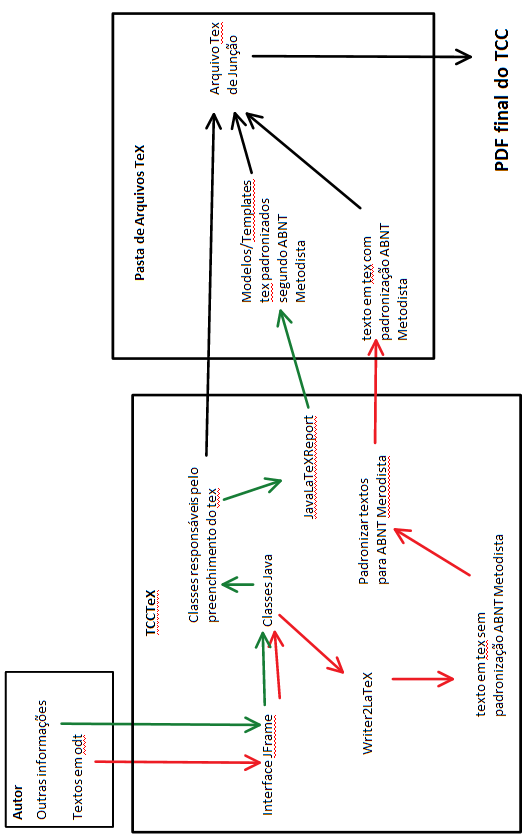
\includegraphics[width=5.49375in,height=8.74028in]{Cap03-img/Cap03-img004.png} 
\fonte{Autoria pr\'opria}} 
\end{figure}

{



\bigskip

\section{FUNCIONAMENTO DO TCCTEX}

\bigskip

{
Neste\ subcap\'itulo explicaremos o funcionamento do software TCCTeX.}

{
O programa se estrutura em 4 pacotes, pacotes de c\'odigos-fonte (padr\~ao do java), pacotes de teste, bibliotecas
(padr\~ao do java), bibliotecas de testes.\ }


\bigskip

{


\begin{figure}[H]
\caption{Projeto \ TCCTeX}}
 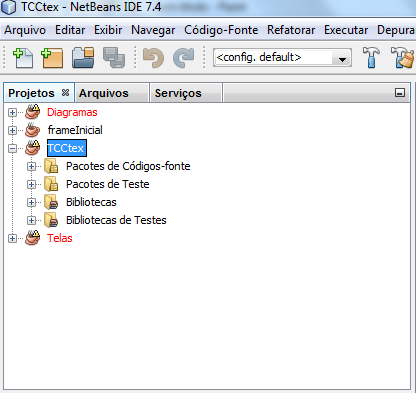
\includegraphics[width=5.22083in,height=4.09097in]{Cap03-img/Cap03-img005.png} 
\fonte{Autoria pr\'opria}} 
\end{figure}

{



\bigskip

{
Pacotes de c\'odigos-fonte s\~ao utilizados para abrigar os pacotes divididos em responsabilidades, no software TCCTeX
temos 3 pacotes principais, br.metodista.TCCtex, br.metodista.TCCtex.telas, br.metodista.TCCTex.telas.imagens.}




{


\begin{figure}[H]
\caption{Pacotes do TCCTeX}}
 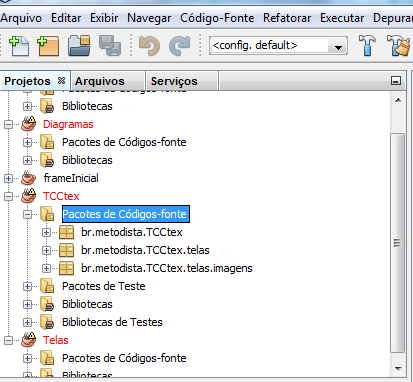
\includegraphics[width=3.94792in,height=3.63611in]{Cap03-img/Cap03-img006.png} 
\fonte{Autoria pr\'opria}} 
\end{figure}




\subsection{Pacote br.metodista.TCCtex}


Este pacote cont\'em as classes java Conversor, Figura, infoEssenciais, PreTextuais, Principal e Textuais.\ 




{


\begin{figure}[H]
\caption{Pacote br.metodista,TCCTeX}
 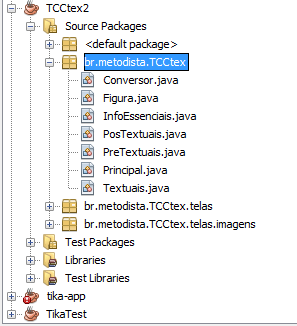
\includegraphics[width=3.09444in,height=3.39653in]{Cap03-img/Cap03-img007.png} 
\fonte{Autoria pr\'opria}} 
\end{figure}

{



\bigskip

\subsubsection{Classe Conversor}

\bigskip

{
Esta classe \'e utilizada para convers\~ao, padroniza\c{c}\~ao e gera\c{c}\~ao de arquivos no formato tex e pdf. Na
classe Conversor, como em todas as outras, se faz necess\'ario a importa\c{c}\~oes de pacotes.}


\bigskip

{


\begin{figure}[H]
\caption{Importa\c{c}\~oes da Classe Conversor}}
 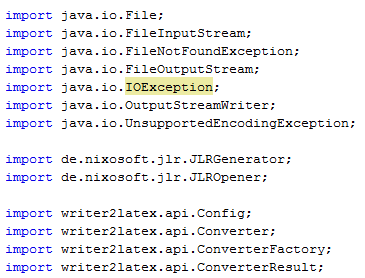
\includegraphics[width=3in,height=2.28333in]{Cap03-img/Cap03-img008.png} 
\fonte{Autoria pr\'opria}} 
\end{figure}

{



\bigskip

{
\textrm{Utilizamos pacotes para organizar as classes, que atuam com um mesmo grupo de caracter\'isticas, o pacote
de.nixosoft.jlr.JLRGenerator por exemplo \'e utilizado no preenchimento de templates feitos em {\LaTeX}, como citado
anteriormente, j\'a o pacote nixosoft.jlr.JLROpener \'e utilizado para convers\~ao de documentos {\LaTeX} para PDF e
possui um m\'etodo open(File) para abrir mais rapidamente o PDF gerado.}}


\bigskip

{


\begin{figure}[H]
\caption{JLR para Gera\c{c}\~ao de PDF}}
 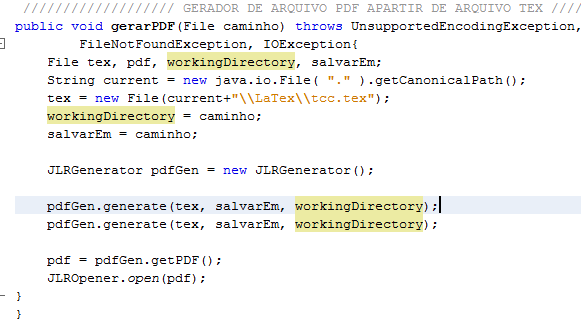
\includegraphics[width=4.34306in,height=2.43264in]{Cap03-img/Cap03-img009.png} 
\fonte{Autoria pr\'opria}} 
\end{figure}

{



\bigskip

{
O pacote writer2latex.api possui a classe\ \textit{Config\ }que armazena o local do arquivo xml de configura\c{c}\~ao do
writer2{\LaTeX} e algumas de suas configura\c{c}\~oes podem ser escritas diretamente na classe java como no exemplo
abaixo onde config.setOption(``inpuntencoding'',''UTF-8'') significa que os arquivos ODT devem ser abertos utilizando o
padr\~ao de codifica\c{c}\~ao UTF-8.}


\bigskip

{


\begin{figure}[H]
\caption{M\'etodo odtToTex}}
 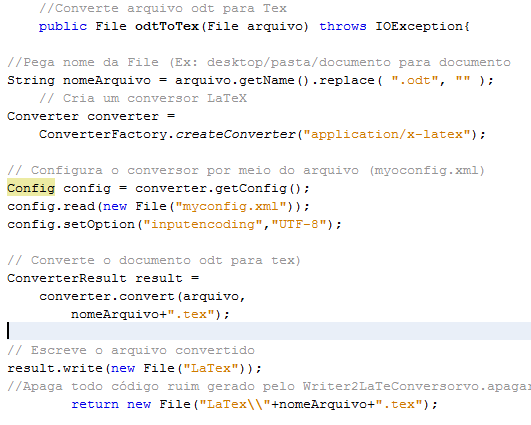
\includegraphics[width=3.88333in,height=3.10417in]{Cap03-img/Cap03-img010.png} 
\fonte{Autoria pr\'opria}} 
\end{figure}

{



\bigskip

{
A classe\ \textit{Converter}\ \'e utilizada para convers\~ao do arquivo ODT para um texto no padr\~ao {\LaTeX}, \ j\'a a
classe CoverterResult recebe esse texto e o escreve em um\ arquivo com a extens\~ao tex.}


\bigskip

{


\begin{figure}[H]
\caption{Parte do M\'etodo alterarTex()}}
 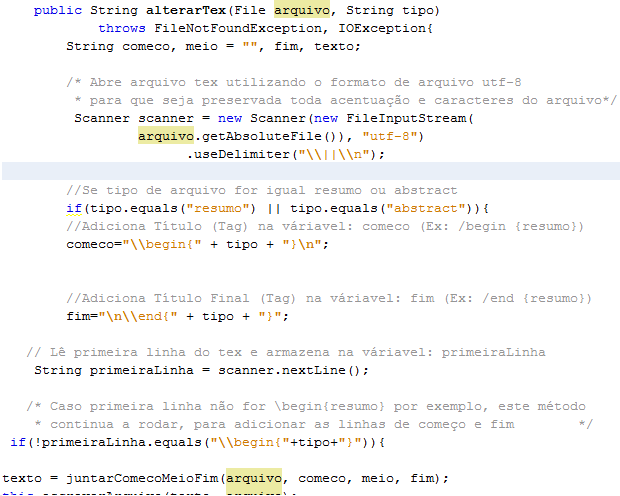
\includegraphics[width=4.62361in,height=3.68819in]{Cap03-img/Cap03-img011.png} 
\fonte{Autoria pr\'opria}} 
\end{figure}

{



\bigskip

{
Seguindo na classe Conversor, temos um outro m\'etodo, chamado alterarTex(), que possui algumas fun\c{c}\~oes como ler o
arquivo convertido pelo Writer2{\LaTeX}, verificar\ se o arquivo \'e o resumo, abstract, dedicat\'oria, etc, adicionar
o t\'itulo se necess\'ario conforme o tipo de arquivo e utilizar outros m\'etodos para remover c\'odigo desnecess\'ario
gerado pelo Writer2{\LaTeX} e reescrever o arquivo tex.}


\bigskip

\subsubsection{Classe InfoEssenciais}

\bigskip

{
A classe InfoEssenciais recebe v\'arias informa\c{c}\~oes necess\'arias para gera\c{c}\~ao da capa, folha de rosto e
folha de aprova\c{c}\~ao, al\'em de gerar uma ficha catalogr\'afica n\~ao preenchida para que pr\'evias do TCC possam
ser entregues, no pr\'oximo exemplo \'e demonstrado um m\'etodo utilizado para gera\c{c}\~ao desses arquivos.}


\bigskip

{


\begin{figure}[H]
\caption{JLR para Preenchimento de Template Tex}}
 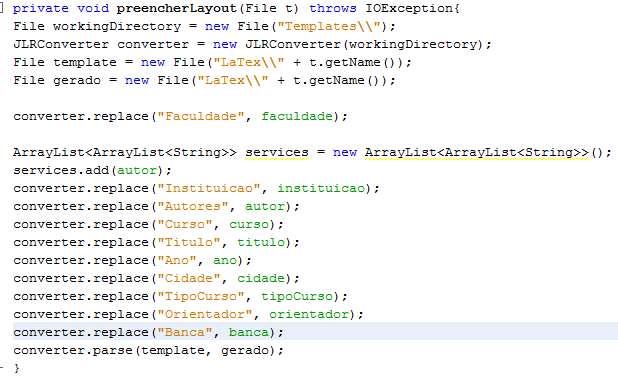
\includegraphics[width=4.85694in,height=2.94792in]{Cap03-img/Cap03-img012.png} 
\fonte{Autoria pr\'opria}} 
\end{figure}

{



\bigskip

\subsubsection{Classe PreTextuais}

\bigskip

{
A classe PreTextuais recebe os arquivos Odt contendo o resumo, abstract, dedicat\'oria, agradecimentos e epigrafe e faz
a convers\~ao dos mesmos para tex se os arquivos obrigat\'orios resumo e abstract existirem.}


\bigskip

{


\begin{figure}[H]
\caption{M\'etodo converterPre()}}
 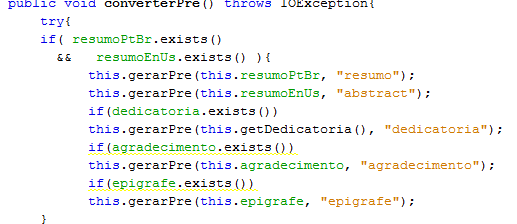
\includegraphics[width=5.38958in,height=2.3375in]{Cap03-img/Cap03-img013.png} 
\fonte{Autoria pr\'opria}} 
\end{figure}

{



\bigskip


\bigskip


\bigskip


\bigskip


\bigskip


\bigskip

\subsubsection{Classe Textuais}

\bigskip

{
A classe Textuais possui algumas vari\'aveis que guardam o caminho de cada arquivo\ utilizado na etapa de Textuais,
s\~ao estas as vari\'aveis introdu\c{c}\~ao e conclus\~ao do tipo\ \textit{File}\ e a lista de cap\'itulos tamb\'em do
tipo\ \textit{File}.}


\bigskip

{


\begin{figure}[H]
\caption{Classe textuais}}
 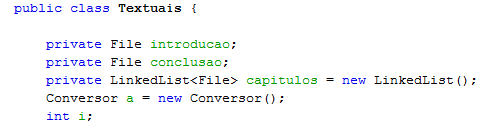
\includegraphics[width=5.14931in,height=1.37292in]{Cap03-img/Cap03-img014.png} 
\fonte{Autoria pr\'opria}} 
\end{figure}

{



\bigskip

{
O m\'etodo listarImagens() da classe Textuais reconhece todas\ legendas de figuras criadas no software Microsoft Word e
coloca no padr\~ao {\LaTeX} corretamente para que possa ser gerada a numera\c{c}\~ao de cada figura e a lista contendo
todas. No pequeno trecho retirado do m\'etodo listarImagens(), mostrado na pr\'oxima figura, \'e\ demonstrado como as
legendas s\~ao reconhecidas pelo software para que posteriormente sejam tratadas e gerado o c\'odigo correto das
mesmas.}


\bigskip


\bigskip

{


\begin{figure}[H]
\caption{M\'etodo converterTextuais()}}
 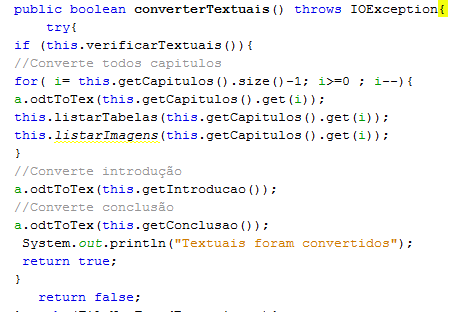
\includegraphics[width=4.31181in,height=2.92222in]{Cap03-img/Cap03-img015.png} 
\fonte{Autoria pr\'opria}} 
\end{figure}

{



\bigskip

\subsubsection{Classe Principal}

\bigskip

{


\begin{figure}[H]
\caption{Parte do m\'etodo abrir() Principal}}
 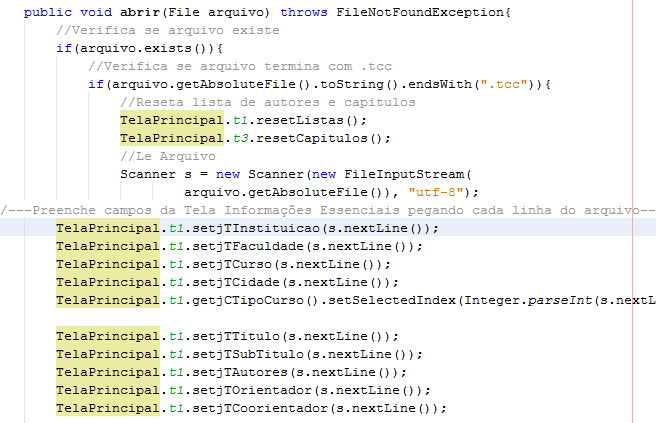
\includegraphics[width=5.90556in,height=3.80934in]{Cap03-img/Cap03-img016.png} 
\fonte{Autoria pr\'opria}} 
\end{figure}

{



\bigskip

{
A Classe principal tem a fun\c{c}\~ao de gerar o arquivo que salva o projeto desenvolvido pelo usu\'ario e de carregar
esse mesmo arquivo, assim o usu\'ario pode salvar o um projeto em andamento e continuar mais tarde.}


\bigskip

\subsection[Pacote\ br.metodista.TCCtex.telas]{Pacote\ br.metodista.TCCtex.telas}

\bigskip

{


\begin{figure}[H]
\caption{Pacote Contendo as Telas}}
 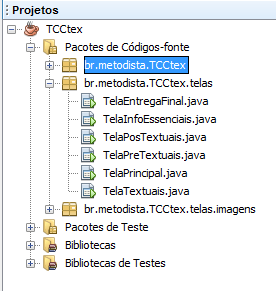
\includegraphics[width=2.36389in,height=2.49375in]{Cap03-img/Cap03-img017.png} 
\fonte{Autoria pr\'opria}} 
\end{figure}

{



\bigskip

{
O pacote br.metodista.TCCtex.telas, possui os formul\'arios da aplica\c{c}\~ao, esses formul\'arios s\~ao JFrames, que
nada mais \'e que uma classe, especializada em componentes visuais, como bot\~oes, menus, caixas de texto, e tudo que
existem em janelas de aplicativos.}


\bigskip

\subsubsection{Pacote br.metodista.TCCTex.telas.imagens}

\bigskip

{


\begin{figure}[H]
\caption{Pacote Contendo Imagens}}
 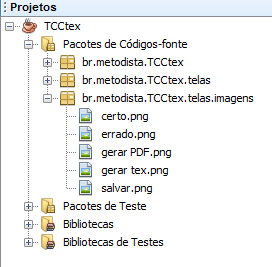
\includegraphics[width=2.22083in,height=2.18194in]{Cap03-img/Cap03-img018.png} 
\fonte{Autoria pr\'opria}} 
\end{figure}

{



\bigskip

{
As boas pr\'aticas da linguagem java, tanto em aplica\c{c}\~oes desktop, quanto WEB, sugerem que os arquivos de imagens
fiquem em um pacote dedicado, na nossa aplica\c{c}\~ao esse pacote \'e o br.metodista.TCCtex.telas.imagens, dentro dele
temos as imagens usadas no aplicativo.}


\bigskip

\section{INTERFACES}

\bigskip

{
O design e funcionamento das interfaces foram feitos de forma a garantir o processo de aprendizagem e uso o mais simples
poss\'ivel, para o usu\'ario final.\ }


\bigskip

\subsection{INTERFACE DA TELA PRINCIPAL}

\bigskip

{
A tela principal \'e composta por: bot\~oes de cada etapa a ser realizada para que o trabalho possa ser
finalizado,\ sendo indicado se determinada etapa foi conclu\'ida ou n\~ao ao seu lado por uma imagem; bot\~ao Salvar,
para guardar todas as informa\c{c}\~oes preenchidas pelo usu\'ario em todas as interfaces gr\'aficas; bot\~ao Gerar PDF
para converter o trabalho gerado de {\LaTeX} para PDF, salvando-o no local onde o usu\'ario desejar.}


\bigskip

{


\begin{figure}[H]
\caption{Interface da Tela Principal}}
 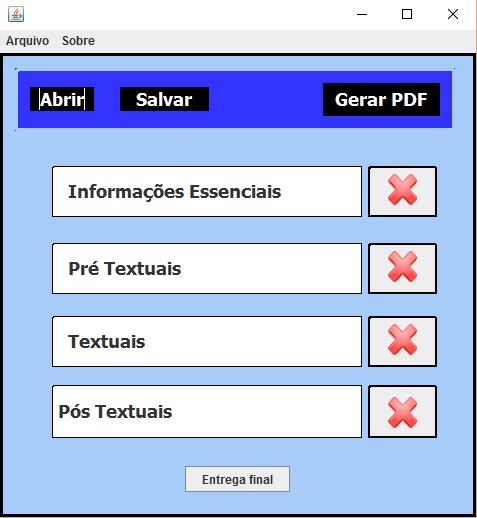
\includegraphics[width=4.97014in,height=5.40278in]{Cap03-img/Cap03-img019.png} 
\fonte{Autoria pr\'opria}} 
\end{figure}

{



\bigskip

{
Quando o usu\'ario conclui determinada etapa a imagem ao lado da op\c{c}\~ao da etapa \'e alterada para indicar que a
mesma foi conclu\'ida.}


\bigskip

{


\begin{figure}[H]
\caption{Etapa Conclu\'ida}}
 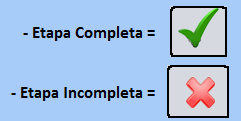
\includegraphics[width=2.50625in,height=1.25972in]{Cap03-img/Cap03-img020.png} 
\fonte{Autoria pr\'opria}} 
\end{figure}

{



\bigskip

\subsection{INTERFACE DA TELA DE INFORMA\c{C}\~OES ESSENCIAIS}

\bigskip

{
A tela de informa\c{c}\~oes essenciais possui os campos de texto: nome da institui\c{c}\~ao, faculdade, curso, cidade da
institui\c{c}\~ao, t\'itulo do trabalho, subt\'itulo, autores, orientador, coorientador(es) e ano de entrega. Tamb\'em
possui o bot\~ao voltar e as caixas de sele\c{c}\~ao: tipo de curso, natureza e terminei esta parte que ao ser clicada
verifica se o usu\'ario preencheu todas informa\c{c}\~oes necess\'arias, caso ele tenha preenchido, s\~ao gerados
arquivos {\LaTeX} para a capa, ficha catalogr\'afica, folha de aprova\c{c}\~ao e folha de rosto, retornando o usu\'ario
para a tela inicial.\ }


\bigskip

{


\begin{figure}[H]
\caption{Interface da Tela de Informa\c{c}\~oes Essenciais}}
 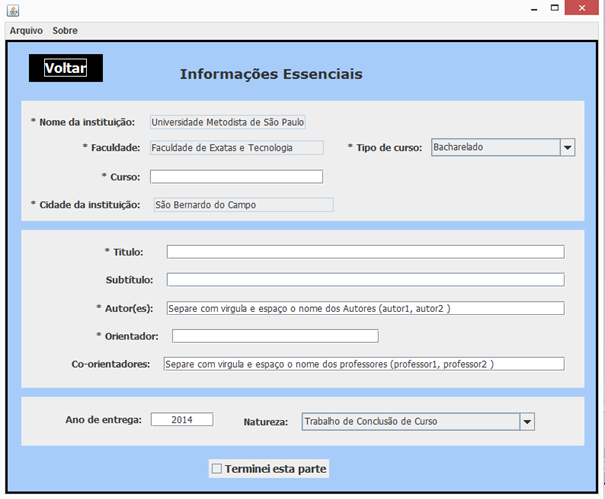
\includegraphics[width=5.83125in,height=4.80486in]{Cap03-img/Cap03-img021.png} 
\fonte{Autoria pr\'opria}} 
\end{figure}

{



\bigskip

\subsection{INTERFACE DA TELA DE PR\'E-TEXTUAIS}

\bigskip


\bigskip

{
Na tela de pr\'e-textuais o usu\'ario dever\'a inserir arquivos com o resumo do trabalho em portugu\^es e ingl\^es
(\textit{abstract}), poder\'a tamb\'em inserir arquivos de texto como a errata, dedicat\'oria, agradecimentos e
epigrafe, sendo que n\~ao dever\'a escrever o t\'itulo de cada parte do trabalho nos documentos. O usu\'ario poder\'a
abrir os documentos ap\'os seleciona-los para efetuar modifica\c{c}\~oes clicando no bot\~ao: abrir. A caixa de
sele\c{c}\~ao: Terminei esta parte ir\'a verificar se o usu\'ario inseriu todos arquivos obrigat\'orios, assim os
convertendo para {\LaTeX} no padr\~ao ABNT utilizado pela metodista.}


\bigskip

{


\begin{figure}[H]
\caption{Interface da tela de Pr\'e-Textuais}}
 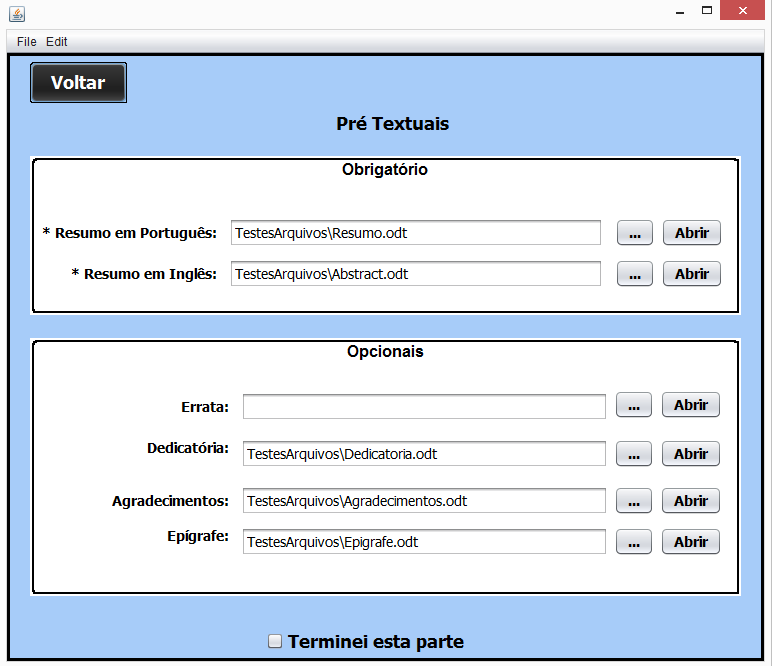
\includegraphics[width=5.73125in,height=4.92569in]{Cap03-img/Cap03-img022.png} 
\fonte{Autoria pr\'opria}} 
\end{figure}

{



\bigskip

\subsection{INTEFACE DA TELA DE TEXTUAIS}

\bigskip

{
Nesta tela o usu\'ario dever\'a inserir arquivos ODT contendo: a introdu\c{c}\~ao, todos cap\'itulos\ separados e
conclus\~ao, o arquivo onde estar\'a escrito cada um, podendo conter tabelas e imagens, tamb\'em poder\'a adicionar
novos cap\'itulos, remove-los e abrir o arquivo para edi\c{c}\~ao.\ }

{
Ao clicar na op\c{c}\~ao: terminei esta parte os arquivos inseridos ser\~ao convertidos para {\LaTeX}, no padr\~ao ABNT
da Metodista.}

{


\begin{figure}[H]
\caption{Interface da Tela de Textuais}}
 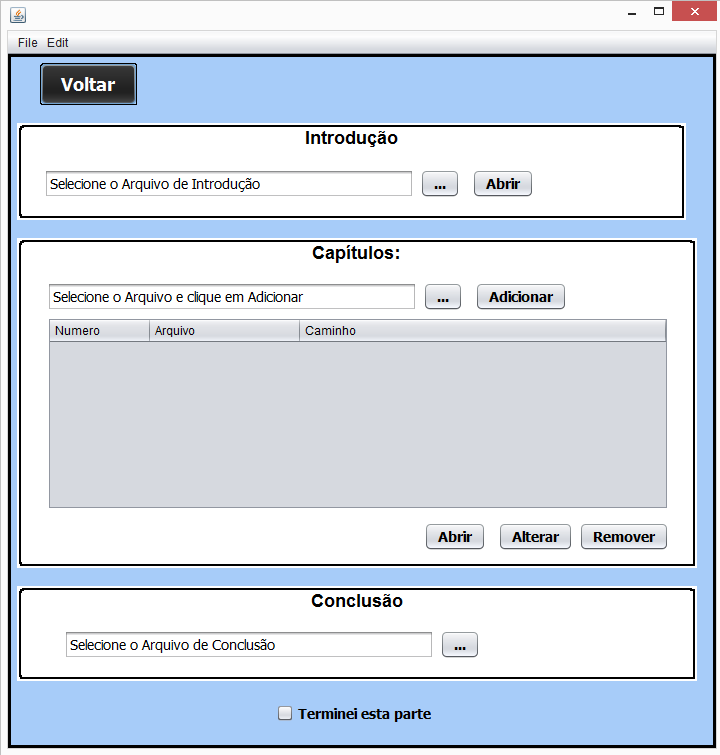
\includegraphics[width=5.75347in,height=6.03889in]{Cap03-img/Cap03-img023.png} 
\fonte{Autoria pr\'opria}} 
\end{figure}

{



\bigskip

\subsection{INTERFACE DA TELA P\'OS-TEXTUAIS}

\bigskip

{
Por meio desta tela ser\'a poss\'ivel inserir um arquivo com todas refer\^encias citadas no texto, para isso o usu\'ario
poder\'a utilizar o sistema Online MORE para criar as cita\c{c}\~oes e refer\^encias e colar as mesmas no documento a
ser inserido. Alguns anexos s\~ao obrigat\'orios, sendo o Relat\'orio de recomenda\c{c}\~oes da banca de
qualifica\c{c}\~ao (RRBQ) um deles. O anexo contendo todas\ Atas e Cronogramas desenvolvidos durante o curso devem ser
estregues no desenvolvimento da entrega final do TCC, sendo assim podem ser adicionados ao documento, caso o usu\'ario
n\~ao esteja fazendo uma pr\'evia do trabalho.}


\bigskip

{


\begin{figure}[H]
\caption{Interface da Tela P\'os-Textuais}}
 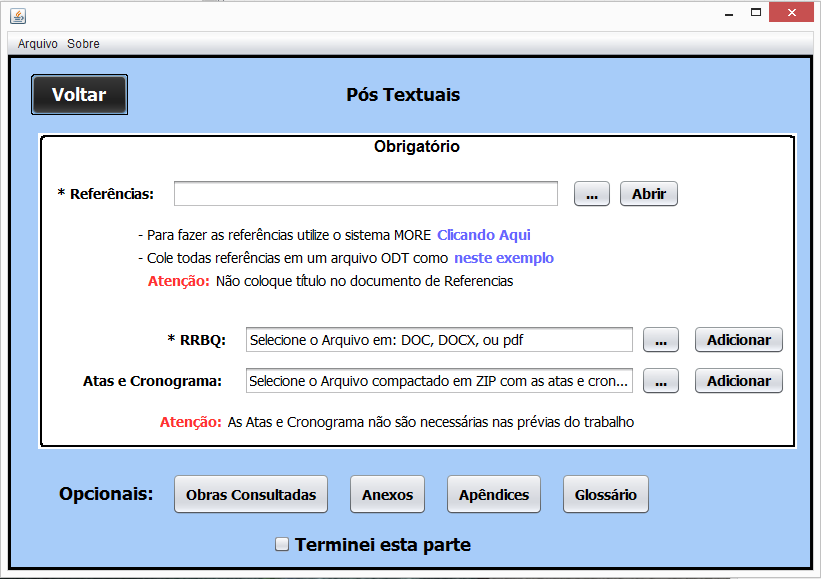
\includegraphics[width=5.89583in,height=4.14931in]{Cap03-img/Cap03-img024.png} 
\fonte{Autoria pr\'opria}} 
\end{figure}

{



\bigskip

\subsection{INTERFACE DA TELA ENTREGA FINAL}

\bigskip

{
A tela de entrega final \'e utilizada apenas como o pr\'oprio nome indica, no desenvolvimento do TCC para entrega final,
para isso o aluno ou seu grupo deve procurar auxilio na biblioteca da Universidade Metodista para produ\c{c}\~ao da
ficha catalogr\'afica, ao enviar algumas informa\c{c}\~oes para a biblioteca como: t\'itulo do trabalho, autores,
orientador, assunto, etc, o aluno receber\'a um documento no qual existir\'a informa\c{c}\~oes como a
classifica\c{c}\~ao de assunto e nota\c{c}\~ao do autor para que o mesmo insira nesta tela e seja gerado o trabalho
para impress\~ao.}


\bigskip

{


\begin{figure}[H]
\caption{Interface da Tela Entrega Final}}
 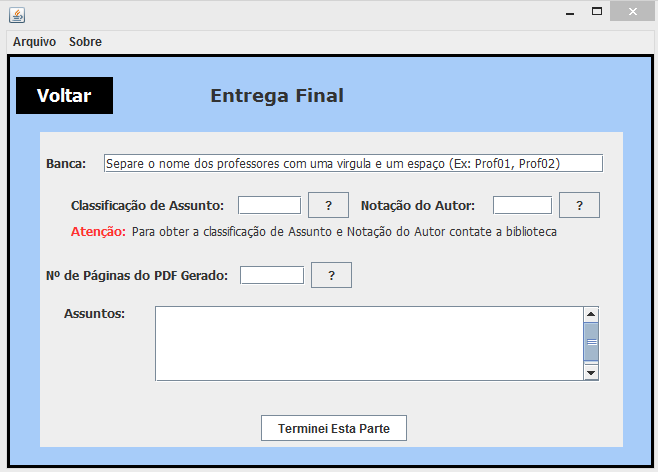
\includegraphics[width=5.90556in,height=4.2354in]{Cap03-img/Cap03-img025.png} 
\fonte{Autoria pr\'opria}} 
\end{figure}

{



\bigskip

\section{REGRAS DE NEG\'OCIO}

\bigskip

{
Aqui estar\~ao listadas algumas regras para que o aluno fa\c{c}a o\ preenchimento da interface:}


\bigskip

{


\begin{center}
\begin{table}
\caption{Regra de Neg\'ocio: Tela Informa\c{c}\~oes Essenciais}}
\tablefirsthead{}

\tablehead{}
\tabletail{}
\tablelasttail{}
\begin{supertabular}{m{1.6837599in}|m{4.04556in}}
\hline
{ Regra de neg\'ocios} &
{ 1}\\\hline
{ Descri\c{c}\~ao}

~

~
 &
{ O aluno deve escrever algumas informa\c{c}\~oes essenciais. Como, nome institui\c{c}\~ao,
faculdade, curso, autores, entres outras.\ }\\\hline
{ Justificativa} &
{ Ao preencher as informa\c{c}\~oes essenciais, \'e gerado um arquivo {\LaTeX} para capa, ficha
catalogr\'afica, folha de aprova\c{c}\~ao e folha de rosto. Caso fosse para inserir arquivos, seria necess\'ario
entradas e telas para cada uma dessas p\'aginas, o que aumentaria o trabalho do aluno}\\\hline
\end{supertabular}
\end{table}
\end{center}
{



\bigskip

{


\begin{center}
\begin{table}
\caption{Regra de Neg\'ocio: Tela Informa\c{c}\~oes Essenciais}}
\tablefirsthead{}

\tablehead{}
\tabletail{}
\tablelasttail{}
\begin{supertabular}{m{1.7003598in}|m{4.06216in}}
\hline
{ Regra de Neg\'ocio} &
{ 2}\\\hline
{ Descri\c{c}\~ao} &
{ Campos em asterisco s\~ao obrigat\'orios.}\\\hline
{ Justificativa} &
{ Informa\c{c}\~oes necess\'arias para os arquivos.}\\\hline
\end{supertabular}
\end{table}
\end{center}
{



\bigskip

{


\begin{center}
\begin{table}
\caption{Regra de Neg\'ocio: Bot\~ao Terminei Esta Parte}}
\tablefirsthead{}

\tablehead{}
\tabletail{}
\tablelasttail{}
\begin{supertabular}{m{1.7191598in}|m{4.0559597in}m{-0.054440156in}}
\hhline{--~}
{ Regra de Neg\'ocio} &
{ 3} &
~
\\\hline
{ Descri\c{c}\~ao} &
\multicolumn{2}{m{4.08026in}}{{ Clicar em terminei esta parte.}}\\\hline
{ Justificativa} &
\multicolumn{2}{m{4.08026in}}{{ Ao clicar nesta marca\c{c}\~ao os arquivos Tex ser\~ao gerados,
e o programa volta para a tela inicial.}}\\\hline
\end{supertabular}
\end{table}
\end{center}
{



\bigskip

{


\begin{center}
\begin{table}
\caption{Regra de Neg\'ocio: Arquivos de Entrada}}
\tablefirsthead{}

\tablehead{}
\tabletail{}
\tablelasttail{}
\begin{supertabular}{m{1.6850599in}|m{4.04626in}}
\hline
{ Regra de Neg\'ocio} &
{ 4}\\\hline
{ Descri\c{c}\~ao\ } &
{ Os arquivos de entradas para transforma\c{c}\~ao no padr\~ao ABNT precisam estar no formato
ODT (Open Document Text) Documento de Texto Aberto.}\\\hline
{ Justificativa} &
{ Por ser Open Source, \'e poss\'ivel\ utilizar junto a v\'arias API's, entre elas o
Writer2Latex a qual estamos usando.}\\\hline
\end{supertabular}
\end{table}
\end{center}
{



\bigskip

{


\begin{center}
\begin{table}
\caption{Regra de Neg\'ocio: Arquivos Opcionais}}
\tablefirsthead{}

\tablehead{}
\tabletail{}
\tablelasttail{}
\begin{supertabular}{m{1.7038599in}|m{4.06496in}}
\hline
{ Regra de Neg\'ocio} &
{ 5}\\\hline
{ Descri\c{c}\~ao} &
{ Arquivos opcionais.}\\\hline
{ Justificativa} &
{ Nem todas as partes de um TCC s\~ao\ obrigat\'orias, algumas s\~ao opcionais como, Errata,
Dedicat\'oria, Ep\'igrafe.}\\\hline
\end{supertabular}
\end{table}
\end{center}
{



\bigskip

{


\begin{center}
\begin{table}
\caption{Regra de Neg\'ocio: Bot\~ao Gerar Tex}}
\tablefirsthead{}

\tablehead{}
\tabletail{}
\tablelasttail{}
\begin{supertabular}{m{1.6934599in}|m{4.0545597in}}
\hline
{ Regra de Neg\'ocio} &
{ 6}\\\hline
{ Descri\c{c}\~ao} &
{ Bot\~ao Gerar Tex funciona apenas se usu\'ario terminou as 4 etapas:
pr\'e-textuais,\ textuais, p\'os-textuais.}\\\hline
{ Justificativa} &
{ Gera os arquivos no formato Tex que poder\'a gerar um arquivo no formato PDF}\\\hline
\end{supertabular}
\end{table}
\end{center}
{



\bigskip

{


\begin{center}
\begin{table}
\caption{Regra de Neg\'ocio: Bot\~ao Gerar PDF}}
\tablefirsthead{}

\tablehead{}
\tabletail{}
\tablelasttail{}
\begin{supertabular}{m{1.7205598in}|m{0.22395986in}m{3.7795599in}}
\hhline{--~}
{ Regra de Neg\'ocio} &
{ 7} &
~
\\\hline
{ Descri\c{c}\~ao} &
\multicolumn{2}{m{4.0822597in}}{{ Bot\~ao Gerar \ PDF funciona se tex foi\ gerado.}}\\\hline
{ Justificativa} &
\multicolumn{2}{m{4.0822597in}}{{ Gera o arquivo no formato pdf. Todas as partes fundamentais
do TCC precisam estar prontas para ser gerado o arquivo.}}\\\hline
\end{supertabular}
\end{table}
\end{center}
{



\bigskip

{


\begin{center}
\begin{table}
\caption{Regra de Neg\'ocio: Adicionar Cap\'itulos da Tela Textuais}}
\tablefirsthead{}

\tablehead{}
\tabletail{}
\tablelasttail{}
\begin{supertabular}{m{1.7177598in}|m{4.07956in}}
\hline
{ Regra de Neg\'ocio} &
{ 8}\\\hline
{ Descri\c{c}\~ao} &
{ Adicionar cap\'itulos}\\\hline
{ Justificativa} &
{ Para que o usu\'ario possa escrever seu arquivo de maneira que achar melhor, n\~ao
necessitando de uma ordem para utilizar o programa.}\\\hline
\end{supertabular}
\end{table}
\end{center}
{



\bigskip

\section{ALTERA\c{C}\~AO DE abnTeX PARA abnTeX2}

\bigskip

{
Para diferenciar a\ vers\~ao original abnTeX do abnTeX2 vamos chamar a vers\~ao original de abnTeX1.}

{
Como o abnTeX1 n\~ao estava catalogada na principal base de dados do {\LaTeX} para utiliza-lo era necess\'ario fazer a
instala\c{c}\~ao manualmente, ainda sim a ultima vers\~ao dispon\'ivel estava\ defasada devido a muitos anos sem
atualiza\c{c}\~oes. Devido a essa defasagem tivemos que adicionar diversos pacotes no arquivo principal do {\LaTeX},
sendo que alguns destes tamb\'em tiveram de ser instalados manualmente para que o pdf final gerado estivesse dentro\ do
padr\~ao ABNT atual. Todo este processo de instala\c{c}\~ao manual de pacotes {\LaTeX} traria grande dificuldade aos
usu\'arios do TCCTeX que nunca haviam utilizado o {\LaTeX} e at\'e mesmo os mais habituados ao {\LaTeX} teriam
dificuldades.}

{
\textrm{Com a altera\c{c}\~ao para o abnTeX2\ estes pacotes n\~ao s\~ao mais necess\'arios pois todos os pacotes
necess\'arios para a formata\c{c}\~ao do documento, bem como o abnTeX2, est\~ao dispon\'iveis do CTAN (Comprehensive
TEX Archive Network) que \'e uma base de dados que possui todo tipo de materiais referentes\ a TeX.\ {}``As principais
distribui\c{c}\~oes LATEX\ s\~ao constru\'idas \`a partir de pacotes e classes do CTAN'' (ARAUJO,2015).}}

{
Com a utiliza\c{c}\~ao do ABNTeX1 houve uma dificuldade maior de aprendizado, pois no site do mesmo n\~ao haviam mais
manuais atualizados de como utiliza-lo e modifica-lo, sendo que tivemos que corrigir diversos problemas do mesmo
reescrevendo diversos comandos.}

{
Com a altera\c{c}\~ao, o c\'odigo fonte do TCCTeX foi alterado em diversos aspectos, removendo coisas desnecess\'arias e
atualizando alguns m\'etodos, como por exemplo m\'etodos relacionados a identifica\c{c}\~ao de figuras, tabelas e o que
deve gerar o arquivo principal com a extens\~ao .tex que conecta todos os outros arquivos tex que formam o documento
PDF do trabalho no padr\~ao ABNT.}

{
Um bom exemplo das modifica\c{c}\~oes que foram feitas no c\'odigo do programa para que ele funcione com abnTeX2 s\~ao
as modifica\c{c}\~oes feitas para a capa e folha de rosto. Como o abnTeX1 estava defasado em rela\c{c}\~ao as ultimas
vers\~oes das normas ABNT era necess\'ario criar templates espec\'ificos para a\ capa e folha de rosto colocando-as na
vers\~ao mais recente das normas ABNT.}

{
Abaixo voc\^e pode verificar uma figura qual era o resultado do preenchimento do template da capa, que gerava o arquivo
``capa.tex'':}


\bigskip

{


\begin{figure}[H]
\caption{Capa em abnTeX1}}
 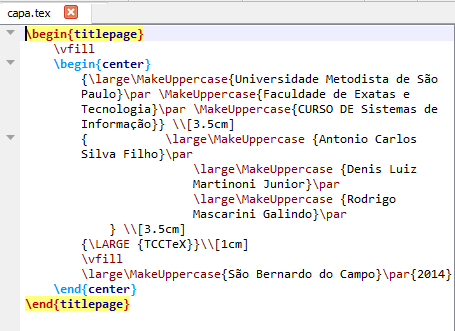
\includegraphics[width=4.74444in,height=3.45347in]{Cap03-img/Cap03-img026.png} 
\fonte{Autoria pr\'opria}} 
\end{figure}

{



\bigskip

{
Abaixo voc\^e pode verificar uma figura qual era o resultado do preenchimento do template da folha de rosto, que gerava
o arquivo ``folharosto.tex'':}


\bigskip

{


\begin{figure}[H]
\caption{Folha de Rosto em abnTeX1}}
 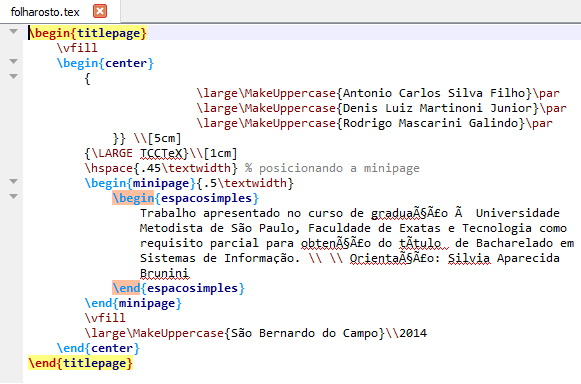
\includegraphics[width=5.89514in,height=3.89514in]{Cap03-img/Cap03-img027.png} 
\fonte{Autoria pr\'opria}} 
\end{figure}

{



\bigskip

{
Quando utilizamos o abnTeX2 s\'o precisamos\ fazer o programa preencher uma s\'erie de macros de dados do documento no
arquivo principal.tex que \'e utilizado para unir todos os arquivos do documento. A figura abaixo mostra como s\~ao
preenchidos esse macros no arquivo principal.tex:}


\bigskip

{


\begin{figure}[H]
\caption{Preenchimento de Macros em principal.tex abnTeX2}}
 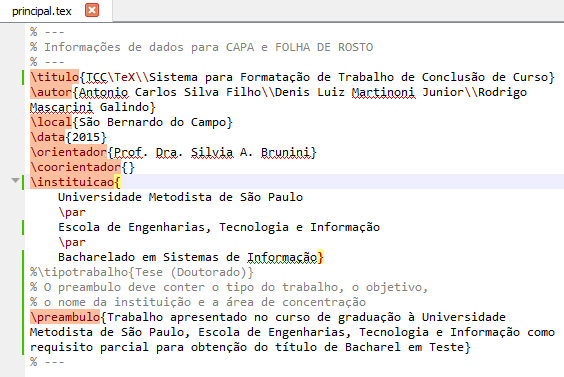
\includegraphics[width=5.88056in,height=3.92569in]{Cap03-img/Cap03-img028.png} 
\fonte{Autoria pr\'opria}} 
\end{figure}

{



\bigskip

{
Ap\'os preencher todos os macros basta utilizar os comandos {\textbackslash}imprimircapa para gerar a capa e
{\textbackslash}imprimirfolhaderosto para gerar a folha de rosto. Esses comandos s\~ao inseridos no pr\'oprio arquivo
principal.tex.}


\bigskip

\section[EXTEN\c{C}\~AO DO PRESENTE TRABALHO]{\textrm{EXTEN\c{C}\~AO DO PRESENTE TRABALHO}}

\bigskip

{
Ap\'os terminar essa fase de desenvolver o software para que ele transforme arquivos em odt para {\LaTeX} colocando-os
dentro dos padr\~oes ABNT, pretendemos desenvolver a mesma funcionalidade para\ transformar arquivos docx em {\LaTeX}
como uma extens\~ao deste projeto.}

{
Para fazer a transforma\c{c}\~ao de textos .docx para um arquivo .tex necessitamos reconhecer os padr\~oes do c\'odigo
xml utilizado pelo docx e comparar com a linguagem {\LaTeX}. Para isso escrevemos\ no Microsoft Word arquivos em docx
com possuem diferentes formata\c{c}\~oes de texto, tabela, imagem e divis\~ao de cap\'itulos, tudo fora da
formata\c{c}\~ao da norma ABNT.\ }


\bigskip

{


\begin{figure}[H]
\caption{Pequeno Texto feito no Microsoft Word}}
 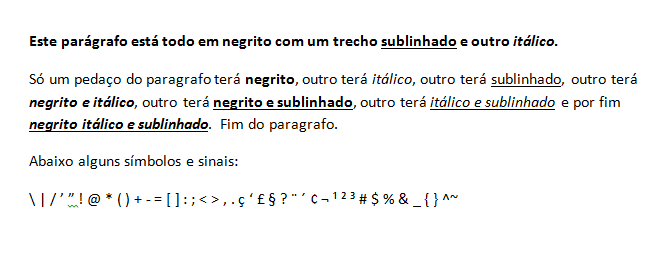
\includegraphics[width=5.90556in,height=2.23174in]{Cap03-img/Cap03-img029.png} 
\fonte{Autoria pr\'opria}} 
\end{figure}

{



\bigskip

{
Em seguida escrevemos, com linguagem {\LaTeX} e utilizando o pacote abnTeX2, arquivos .tex com o mesmo conte\'udo dos
arquivos .docx, por\'em obedecendo as normas abnt.}


\bigskip

{


\begin{figure}[H]
\caption{Pequeno texto em {\LaTeX} com mesmo conte\'udo da figura anterior}}
 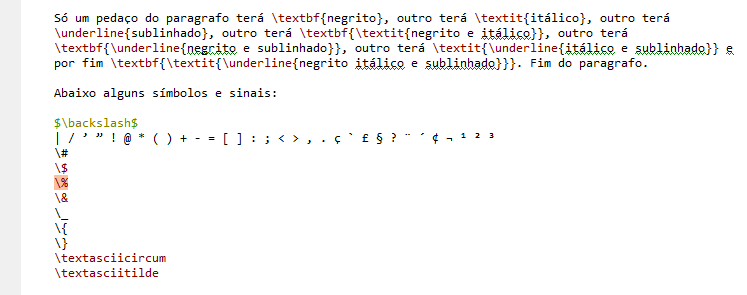
\includegraphics[width=5.90556in,height=2.33366in]{Cap03-img/Cap03-img030.png} 
\fonte{Autoria pr\'opria}} 
\end{figure}

{



\bigskip

{
Em seguida fazemos uma c\'opia do arquivo docx e renomeamos a extens\~ao dessa c\'opia para .zip para assim podermos
descompactar os arquivos xml do docx.}

{
Ap\'os descompactar os arquivos .docx, abrimos, utilizando o NetBeans IDE, o arquivo document.xml que possui o parte
principal do c\'odigo xml\ }


\bigskip

{


\begin{figure}[H]
\caption{Pequena parte do c\'odigo XML do docx}}
 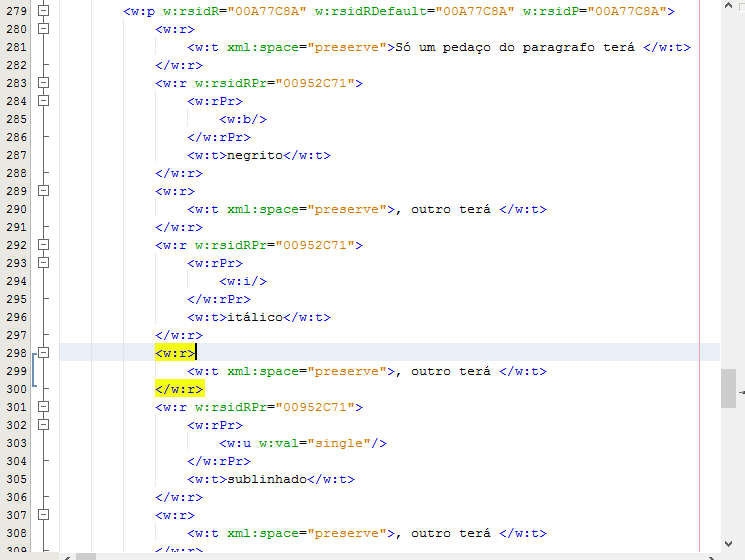
\includegraphics[width=5.90556in,height=4.43403in]{Cap03-img/Cap03-img031.png} 
\fonte{Autoria pr\'opria}} 
\end{figure}

{



\bigskip

{
Este arquivo document.xml \'e bastante extenso e possui todo o conte\'udo inserido no arquivo docx. Cada arquivo docx
possui seu pr\'oprio arquivo document.xml.}

{
\textrm{A partir\ disso teremos que, utilizando o NetBeans IDE, reconhecer os padr\~oes da linguagem xml utilizada no
arquivo .docx, compar\'a-los com os padr\~oes da liguagem {\LaTeX} utilizada no arquivo .tex e criar est\'orias de como
o c\'odigo Java ir\'a converter os arquivos de uma\ linguagem para outra. A partir dessas est\'orias ser\'a criado o
conversor de .docx para {\LaTeX} em Java.\ }}